% ==================== UNIDAD II ====================
% Derivadas Parciales

\section{Unidad II: Derivadas Parciales}

\begin{TemaBox}[Derivadas Parciales: Concepto fundamental]
Las derivadas parciales extienden el concepto de derivada a funciones de varias variables, permitiéndonos estudiar cómo cambia una función cuando variamos una sola variable mientras mantenemos las demás constantes. Este concepto es fundamental en física, ingeniería, economía y todas las áreas donde interactúan múltiples variables.
\end{TemaBox}

\subsection{La derivada parcial}

\paragraph{Introducción.}
En cálculo de una variable, la derivada \(\frac{dy}{dx}\) mide la razón de cambio de \(y\) con respecto a \(x\). Para funciones de varias variables, necesitamos un concepto similar que nos permita medir cómo cambia la función cuando variamos una variable a la vez.

Consideremos una función \(z = f(x,y)\) de dos variables. Podemos estudiar cómo cambia \(z\) cuando:
\begin{itemize}
  \item Variamos \(x\) manteniendo \(y\) constante
  \item Variamos \(y\) manteniendo \(x\) constante
\end{itemize}

\begin{InfoBox}
\Meta{Definición}{La \textbf{derivada parcial} de \(f\) con respecto a \(x\) se denota \(\frac{\partial f}{\partial x}\) o \(f_x\), y se calcula derivando con respecto a \(x\) tratando \(y\) como constante.}

\Meta{Notación}{Para \(z = f(x,y)\) usamos:}
\begin{itemize}
  \item \(\frac{\partial f}{\partial x}\), \(\frac{\partial z}{\partial x}\), \(f_x(x,y)\), o \(z_x\)
  \item \(\frac{\partial f}{\partial y}\), \(\frac{\partial z}{\partial y}\), \(f_y(x,y)\), o \(z_y\)
\end{itemize}
\end{InfoBox}

\paragraph{Definición formal.}
Sea \(z = f(x,y)\) una función de dos variables. Las derivadas parciales se definen como:

\[
\frac{\partial f}{\partial x} = \lim_{h \to 0} \frac{f(x+h, y) - f(x,y)}{h}
\]

\[
\frac{\partial f}{\partial y} = \lim_{h \to 0} \frac{f(x, y+h) - f(x,y)}{h}
\]

\paragraph{Interpretación geométrica.}
\begin{itemize}
  \item \(\frac{\partial f}{\partial x}\) representa la pendiente de la curva formada al intersectar la superficie \(z=f(x,y)\) con un plano \(y=\text{constante}\)
  \item \(\frac{\partial f}{\partial y}\) representa la pendiente de la curva formada al intersectar la superficie \(z=f(x,y)\) con un plano \(x=\text{constante}\)
\end{itemize}

\paragraph{Ejemplos resueltos.}

\begin{EjercicioBox}[Ejemplo 1: Función polinomial]
Calcular las derivadas parciales de \(f(x,y) = x^3 + 2xy^2 - y^3\).

\textbf{Solución:}

\textbf{Para} \(\frac{\partial f}{\partial x}\): Tratamos \(y\) como constante
\begin{align*}
\frac{\partial f}{\partial x} &= \frac{\partial}{\partial x}(x^3 + 2xy^2 - y^3) \\
&= 3x^2 + 2y^2 \cdot 1 - 0 \\
&= \boxed{3x^2 + 2y^2}
\end{align*}

\textbf{Para} \(\frac{\partial f}{\partial y}\): Tratamos \(x\) como constante
\begin{align*}
\frac{\partial f}{\partial y} &= \frac{\partial}{\partial y}(x^3 + 2xy^2 - y^3) \\
&= 0 + 2x \cdot 2y - 3y^2 \\
&= \boxed{4xy - 3y^2}
\end{align*}
\end{EjercicioBox}

\begin{EjercicioBox}[Ejemplo 2: Función con exponencial]
Calcular las derivadas parciales de \(f(x,y) = e^{xy} + \sin(x) \cos(y)\).

\textbf{Solución:}

\textbf{Para} \(\frac{\partial f}{\partial x}\):
\begin{align*}
\frac{\partial f}{\partial x} &= \frac{\partial}{\partial x}(e^{xy} + \sin(x)\cos(y)) \\
&= e^{xy} \cdot y + \cos(x) \cdot \cos(y) \\
&= \boxed{ye^{xy} + \cos(x)\cos(y)}
\end{align*}

\textbf{Para} \(\frac{\partial f}{\partial y}\):
\begin{align*}
\frac{\partial f}{\partial y} &= \frac{\partial}{\partial y}(e^{xy} + \sin(x)\cos(y)) \\
&= e^{xy} \cdot x + \sin(x) \cdot (-\sin(y)) \\
&= \boxed{xe^{xy} - \sin(x)\sin(y)}
\end{align*}
\end{EjercicioBox}

\begin{EjercicioBox}[Ejemplo 3: Función racional]
Calcular las derivadas parciales de \(f(x,y) = \frac{x^2 + y^2}{x - y}\).

\textbf{Solución:}

\textbf{Para} \(\frac{\partial f}{\partial x}\): Usamos la regla del cociente
\begin{align*}
\frac{\partial f}{\partial x} &= \frac{(x-y)\frac{\partial}{\partial x}(x^2+y^2) - (x^2+y^2)\frac{\partial}{\partial x}(x-y)}{(x-y)^2} \\
&= \frac{(x-y)(2x) - (x^2+y^2)(1)}{(x-y)^2} \\
&= \frac{2x^2 - 2xy - x^2 - y^2}{(x-y)^2} \\
&= \boxed{\frac{x^2 - 2xy - y^2}{(x-y)^2}}
\end{align*}

\textbf{Para} \(\frac{\partial f}{\partial y}\):
\begin{align*}
\frac{\partial f}{\partial y} &= \frac{(x-y)\frac{\partial}{\partial y}(x^2+y^2) - (x^2+y^2)\frac{\partial}{\partial y}(x-y)}{(x-y)^2} \\
&= \frac{(x-y)(2y) - (x^2+y^2)(-1)}{(x-y)^2} \\
&= \frac{2xy - 2y^2 + x^2 + y^2}{(x-y)^2} \\
&= \boxed{\frac{x^2 + 2xy - y^2}{(x-y)^2}}
\end{align*}
\end{EjercicioBox}

\begin{EjercicioBox}[Ejemplo 4: Función de tres variables]
Calcular las derivadas parciales de \(f(x,y,z) = x^2yz + xy^2z + xyz^2\).

\textbf{Solución:}

\textbf{Para} \(\frac{\partial f}{\partial x}\):
\begin{align*}
\frac{\partial f}{\partial x} &= 2xyz + y^2z + yz^2 = \boxed{yz(2x + y + z)}
\end{align*}

\textbf{Para} \(\frac{\partial f}{\partial y}\):
\begin{align*}
\frac{\partial f}{\partial y} &= x^2z + 2xyz + xz^2 = \boxed{xz(x + 2y + z)}
\end{align*}

\textbf{Para} \(\frac{\partial f}{\partial z}\):
\begin{align*}
\frac{\partial f}{\partial z} &= x^2y + xy^2 + 2xyz = \boxed{xy(x + y + 2z)}
\end{align*}
\end{EjercicioBox}

\paragraph{Aplicaciones prácticas.}
Las derivadas parciales tienen aplicaciones en:
\begin{itemize}
  \item \textbf{Física:} Ecuaciones de calor, ondas y difusión
  \item \textbf{Economía:} Utilidad marginal, productividad marginal
  \item \textbf{Ingeniería:} Análisis de sensibilidad en diseño
  \item \textbf{Estadística:} Optimización de funciones de verosimilitud
  \item \textbf{Machine Learning:} Gradiente descendente en redes neuronales
\end{itemize}

\subsubsection{Construcción geométrica de la derivada parcial con software}

\begin{TemaBox}[Visualización geométrica de derivadas parciales]
La interpretación geométrica de las derivadas parciales nos permite comprender cómo se comporta una superficie tridimensional al realizar cortes paralelos a los planos coordenados. Cada derivada parcial representa la pendiente de una curva resultante de estas intersecciones.
\end{TemaBox}

\paragraph{Concepto geométrico fundamental.}

Para una función \(z = f(x,y)\) que representa una superficie en el espacio tridimensional:

\begin{itemize}
  \item \(\frac{\partial f}{\partial x}\) en \((x_0, y_0)\) es la pendiente de la curva de intersección entre la superficie y el plano \(y = y_0\)
  \item \(\frac{\partial f}{\partial y}\) en \((x_0, y_0)\) es la pendiente de la curva de intersección entre la superficie y el plano \(x = x_0\)
\end{itemize}

\paragraph{Visualización paso a paso.}

Consideremos la función \(f(x,y) = x^2 + y^2\) (un paraboloide). Vamos a visualizar cómo se construyen geométricamente sus derivadas parciales.

\begin{figure}[h!]
\centering
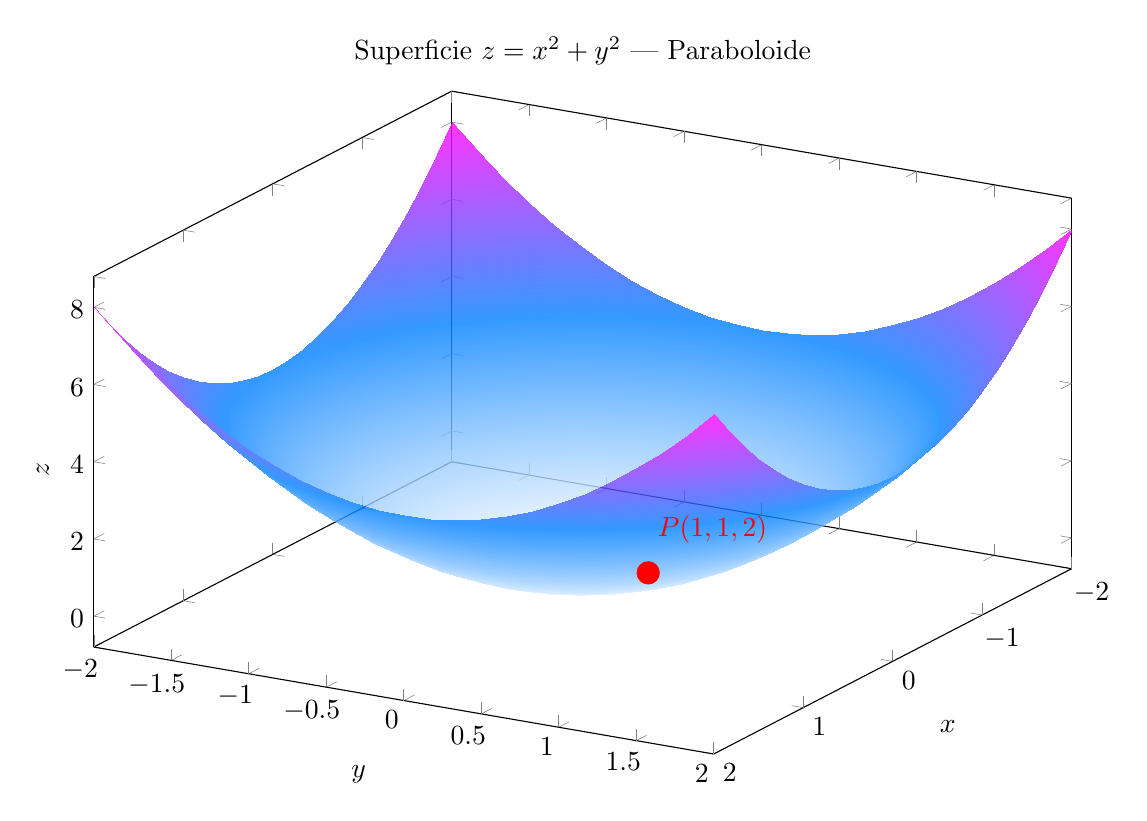
\begin{tikzpicture}
  \begin{axis}[
      view={120}{30},
      width=14cm, height=10cm,
      xlabel={$x$}, ylabel={$y$}, zlabel={$z$},
      domain=-2:2, y domain=-2:2,
      samples=25, samples y=25,
      colormap/cool,
      title={Superficie \(z = x^2 + y^2\) — Paraboloide}
  ]
    % Superficie principal
    \addplot3[surf,opacity=0.8,shader=interp] {x^2 + y^2};
    
    % Punto de interés
    \addplot3[only marks, mark=*, mark size=4pt, color=red] coordinates {(1,1,2)};
    \node[anchor=south west] at (axis cs:1,1,2.5) {\textcolor{red}{$P(1,1,2)$}};
  \end{axis}
\end{tikzpicture}
\caption{Superficie \(z = f(x,y) = x^2 + y^2\) con punto de interés \(P(1,1,2)\).}
\label{fig:superficie_base}
\end{figure}

\paragraph{Derivada parcial respecto a \(x\): Corte con \(y = \text{constante}\).}

Cuando fijamos \(y = 1\), la superficie se reduce a una curva en el plano \(y = 1\):
\[
z = f(x,1) = x^2 + 1
\]

La derivada parcial en \((1,1)\) es:
\[
\frac{\partial f}{\partial x}\bigg|_{(1,1)} = 2x\bigg|_{x=1} = 2
\]

Esto significa que la pendiente de la curva en el punto \(P\) es 2 cuando nos movemos en la dirección \(x\).

\begin{figure}[h!]
\centering
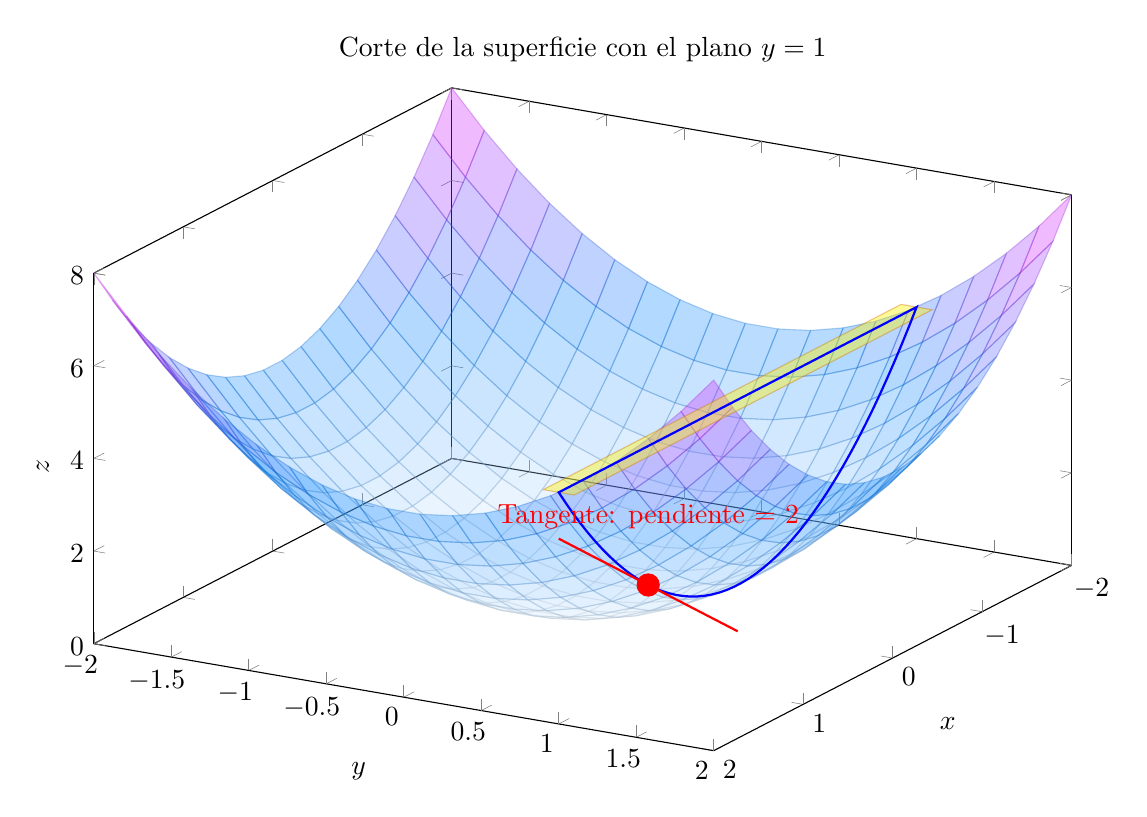
\begin{tikzpicture}
  \begin{axis}[
      view={120}{30},
      width=14cm, height=10cm,
      xlabel={$x$}, ylabel={$y$}, zlabel={$z$},
      xmin=-2, xmax=2, ymin=-2, ymax=2, zmin=0, zmax=8,
      title={Corte de la superficie con el plano \(y=1\)}
  ]
    % Superficie translúcida
    \addplot3[surf,opacity=0.3,colormap/cool,domain=-2:2, y domain=-2:2,samples=20] {x^2 + y^2};
    
    % Plano y=1
    \addplot3[surf,opacity=0.4,color=yellow,domain=-2:2,y domain=0.9:1.1,samples=2] {x^2 + 1};
    
    % Curva de intersección y=1
    \addplot3[thick,color=blue,domain=-2:2,samples=50] (x,1,{x^2 + 1});
    
    % Punto de tangencia
    \addplot3[only marks, mark=*, mark size=4pt, color=red] coordinates {(1,1,2)};
    
    % Recta tangente con pendiente 2
    \addplot3[thick,color=red,domain=0:2,samples=2] (x,1,{2*(x-1) + 2});
    
    \node[anchor=south] at (axis cs:1,1,3) {\textcolor{red}{Tangente: pendiente = 2}};
  \end{axis}
\end{tikzpicture}
\caption{Curva azul: intersección con \(y=1\). Recta roja: tangente con pendiente \(\frac{\partial f}{\partial x} = 2\).}
\label{fig:corte_x}
\end{figure}

\paragraph{Derivada parcial respecto a \(y\): Corte con \(x = \text{constante}\).}

Cuando fijamos \(x = 1\), la superficie se reduce a:
\[
z = f(1,y) = 1 + y^2
\]

La derivada parcial en \((1,1)\) es:
\[
\frac{\partial f}{\partial y}\bigg|_{(1,1)} = 2y\bigg|_{y=1} = 2
\]

\begin{figure}[h!]
\centering
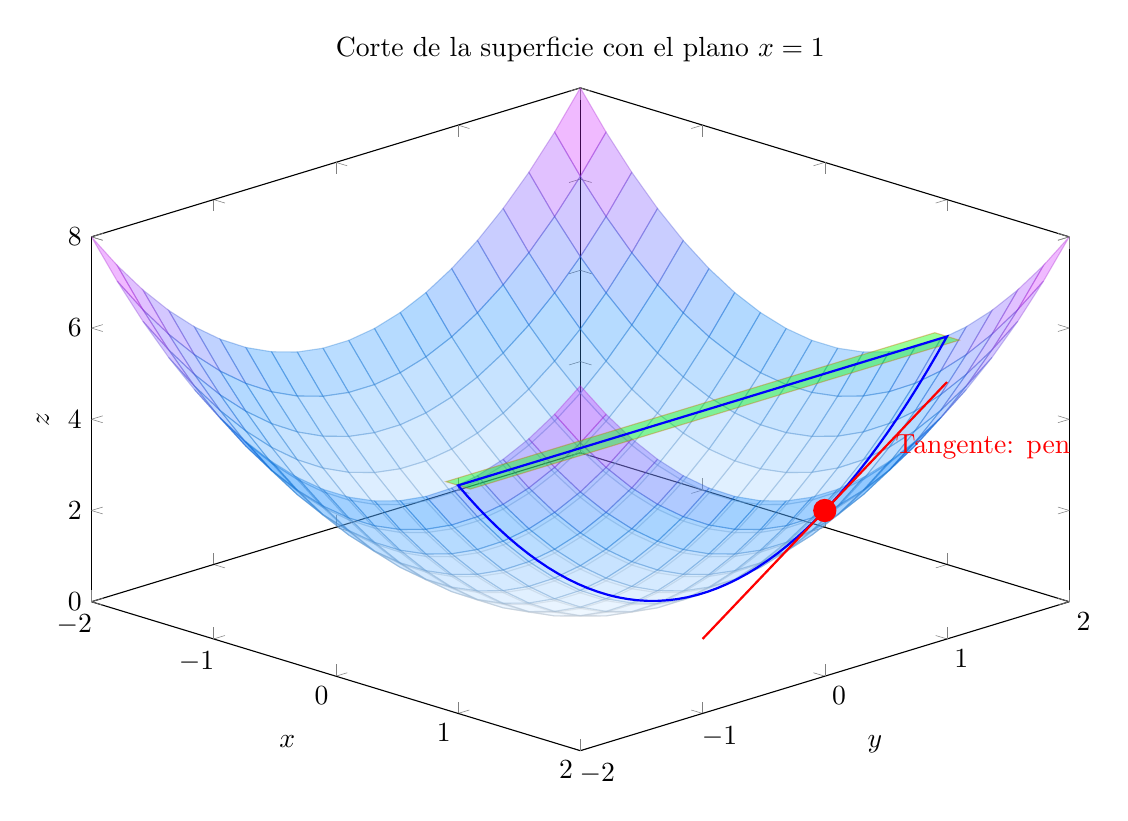
\begin{tikzpicture}
  \begin{axis}[
      view={45}{30},
      width=14cm, height=10cm,
      xlabel={$x$}, ylabel={$y$}, zlabel={$z$},
      xmin=-2, xmax=2, ymin=-2, ymax=2, zmin=0, zmax=8,
      title={Corte de la superficie con el plano \(x=1\)}
  ]
    % Superficie translúcida
    \addplot3[surf,opacity=0.3,colormap/cool,domain=-2:2, y domain=-2:2,samples=20] {x^2 + y^2};
    
    % Plano x=1
    \addplot3[surf,opacity=0.4,color=green,domain=0.9:1.1,y domain=-2:2,samples=2] {1 + y^2};
    
    % Curva de intersección x=1
    \addplot3[thick,color=blue,domain=-2:2,samples=50] (1,x,{1 + x^2});
    
    % Punto de tangencia
    \addplot3[only marks, mark=*, mark size=4pt, color=red] coordinates {(1,1,2)};
    
    % Recta tangente con pendiente 2
    \addplot3[thick,color=red,domain=0:2,samples=2] (1,x,{2*(x-1) + 2});
    
    \node[anchor=west] at (axis cs:1,1.5,3) {\textcolor{red}{Tangente: pendiente = 2}};
  \end{axis}
\end{tikzpicture}
\caption{Curva azul: intersección con \(x=1\). Recta roja: tangente con pendiente \(\frac{\partial f}{\partial y} = 2\).}
\label{fig:corte_y}
\end{figure}

\paragraph{Ejemplo 2: Silla de montar (Paraboloide hiperbólico).}

Consideremos ahora \(f(x,y) = x^2 - y^2\), una superficie con forma de silla de montar.

Calculamos las derivadas parciales:
\[
\frac{\partial f}{\partial x} = 2x, \quad \frac{\partial f}{\partial y} = -2y
\]

En el punto \((1, 1, 0)\):
\[
\frac{\partial f}{\partial x}\bigg|_{(1,1)} = 2, \quad \frac{\partial f}{\partial y}\bigg|_{(1,1)} = -2
\]

\begin{figure}[h!]
\centering
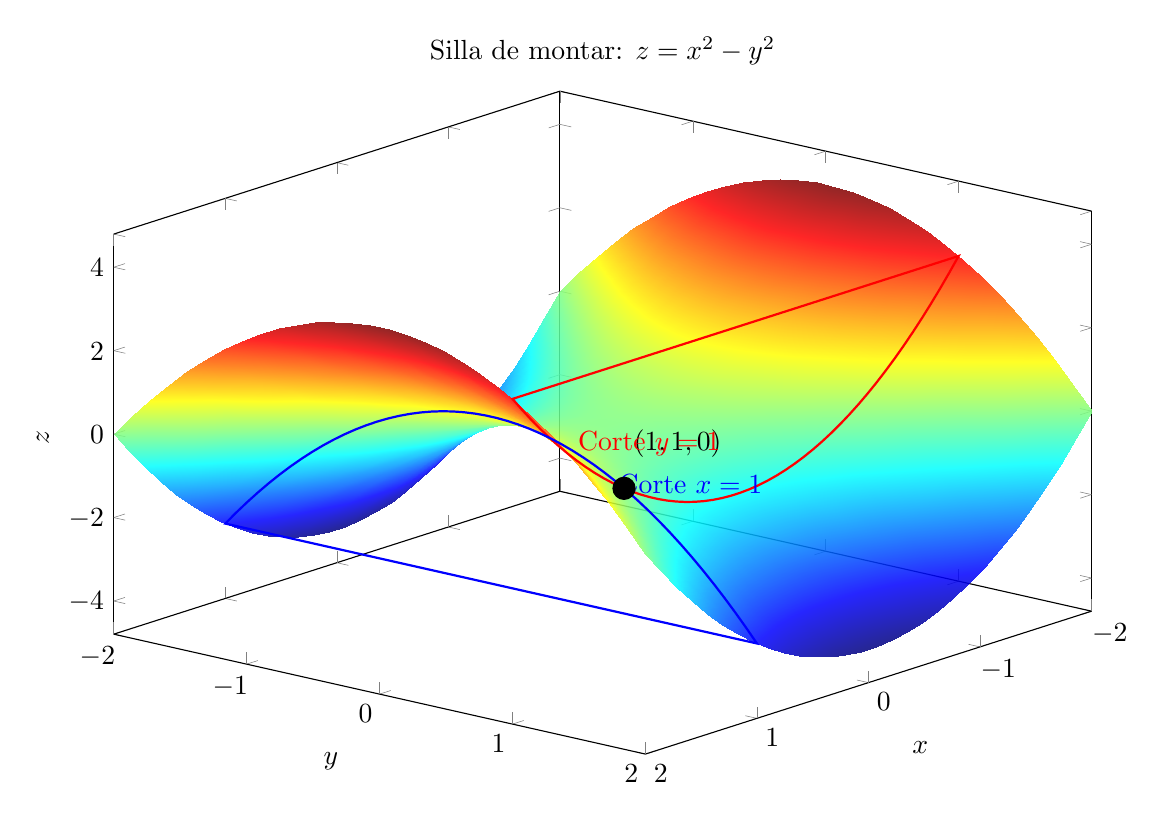
\begin{tikzpicture}
  \begin{axis}[
      view={130}{25},
      width=14cm, height=10cm,
      xlabel={$x$}, ylabel={$y$}, zlabel={$z$},
      domain=-2:2, y domain=-2:2,
      samples=30, samples y=30,
      colormap/jet,
      title={Silla de montar: \(z = x^2 - y^2\)}
  ]
    % Superficie
    \addplot3[surf,opacity=0.85,shader=interp] {x^2 - y^2};
    
    % Punto de interés
    \addplot3[only marks, mark=*, mark size=4pt, color=black] coordinates {(1,1,0)};
    \node[anchor=south west] at (axis cs:1,1,0.5) {$(1,1,0)$};
    
    % Curvas de corte
    \addplot3[thick,color=red,domain=-2:2,samples=50] (x,1,{x^2 - 1});
    \addplot3[thick,color=blue,domain=-2:2,samples=50] (1,x,{1 - x^2});
    
    % Etiquetas de las curvas
    \node[anchor=west,red] at (axis cs:1.5,1,1.5) {Corte $y=1$};
    \node[anchor=south,blue] at (axis cs:1,1.5,0) {Corte $x=1$};
  \end{axis}
\end{tikzpicture}
\caption{Silla de montar con cortes que muestran pendientes opuestas en direcciones perpendiculares.}
\label{fig:silla_montar}
\end{figure}

\paragraph{Comparación visual de curvaturas.}

La siguiente gráfica muestra las curvas de nivel de la función paraboloide. Cada círculo representa puntos donde la función tiene el mismo valor:

\begin{figure}[h!]
\centering
\begin{tikzpicture}
  \begin{axis}[
      axis equal image,
      width=12cm,height=10cm,
      axis lines=middle, xlabel={$x$}, ylabel={$y$},
      xmin=-2.5, xmax=2.5, ymin=-2.5, ymax=2.5,
      grid=both, grid style={gray!20},
      title={Curvas de nivel de \(f(x,y) = x^2 + y^2\)}
  ]
    % Curvas de nivel (círculos concéntricos)
    \addplot[brand,thick,domain=0:360,samples=100] ({cos(x)},{sin(x)});
    \addplot[brand,thick,domain=0:360,samples=100] ({1.414*cos(x)},{1.414*sin(x)});
    \addplot[brand,thick,domain=0:360,samples=100] ({1.732*cos(x)},{1.732*sin(x)});
    \addplot[brand,thick,domain=0:360,samples=100] ({2*cos(x)},{2*sin(x)});
    
    % Puntos de referencia
    \addplot[only marks,mark=*,mark size=3pt,color=red] coordinates {(1,0) (0,1) (1,1)};
    
    % Etiquetas de los puntos
    \node[anchor=west] at (axis cs:1.1,0) {$(1,0)$};
    \node[anchor=south] at (axis cs:0,1.1) {$(0,1)$};
    \node[anchor=south west] at (axis cs:1.1,1.1) {$(1,1)$};
  \end{axis}
\end{tikzpicture}
\caption{Curvas de nivel: círculos concéntricos para $k=1,2,3,4$.}
\label{fig:nivel_vectores}
\end{figure}

\paragraph{Interpretación práctica con software.}

En software como \textbf{GeoGebra}, \textbf{Mathematica}, \textbf{MATLAB} o \textbf{Python} (matplotlib), podemos:

\begin{enumerate}
  \item \textbf{Graficar la superficie} \(z = f(x,y)\) en 3D
  \item \textbf{Crear planos de corte} \(x = x_0\) o \(y = y_0\)
  \item \textbf{Visualizar las curvas de intersección}
  \item \textbf{Calcular y dibujar las rectas tangentes} con pendientes dadas por las derivadas parciales
  \item \textbf{Animar} el movimiento del punto para ver cómo cambian las pendientes
\end{enumerate}

\begin{InfoBox}
\Meta{Herramientas recomendadas}{GeoGebra 3D, Desmos 3D Calculator, Python (matplotlib + numpy), MATLAB, Mathematica, Wolfram Alpha}

\Meta{Ventajas de la visualización}{Permite comprender intuitivamente conceptos abstractos, verificar cálculos analíticos y explorar comportamientos locales de funciones complejas.}
\end{InfoBox}

\paragraph{Ejercicio guiado con visualización.}

\begin{EjercicioBox}[Ejercicio: Cono]
Considera la función \(f(x,y) = \sqrt{x^2 + y^2}\), que representa un cono.

\textbf{Tareas:}
\begin{enumerate}
  \item Calcula \(\frac{\partial f}{\partial x}\) y \(\frac{\partial f}{\partial y}\)
  \item Evalúa las derivadas en el punto \((3, 4)\)
  \item Interpreta geométricamente el resultado
\end{enumerate}

\textbf{Solución:}

\textbf{1. Cálculo de derivadas parciales:}
\begin{align*}
\frac{\partial f}{\partial x} &= \frac{\partial}{\partial x}\sqrt{x^2 + y^2} = \frac{x}{\sqrt{x^2 + y^2}} = \frac{x}{f(x,y)} \\[0.5em]
\frac{\partial f}{\partial y} &= \frac{\partial}{\partial y}\sqrt{x^2 + y^2} = \frac{y}{\sqrt{x^2 + y^2}} = \frac{y}{f(x,y)}
\end{align*}

\textbf{2. Evaluación en} \((3,4)\):
\[
f(3,4) = \sqrt{9 + 16} = 5
\]
\[
\frac{\partial f}{\partial x}\bigg|_{(3,4)} = \frac{3}{5} = 0.6, \quad \frac{\partial f}{\partial y}\bigg|_{(3,4)} = \frac{4}{5} = 0.8
\]

\textbf{3. Interpretación geométrica:}
\begin{itemize}
  \item Al movernos en dirección \(x\) desde \((3,4,5)\), la superficie sube con pendiente 0.6
  \item Al movernos en dirección \(y\), la pendiente es 0.8
  \item Ambas pendientes son positivas porque nos alejamos del vértice del cono en el origen
\end{itemize}
\end{EjercicioBox}

\begin{figure}[h!]
\centering
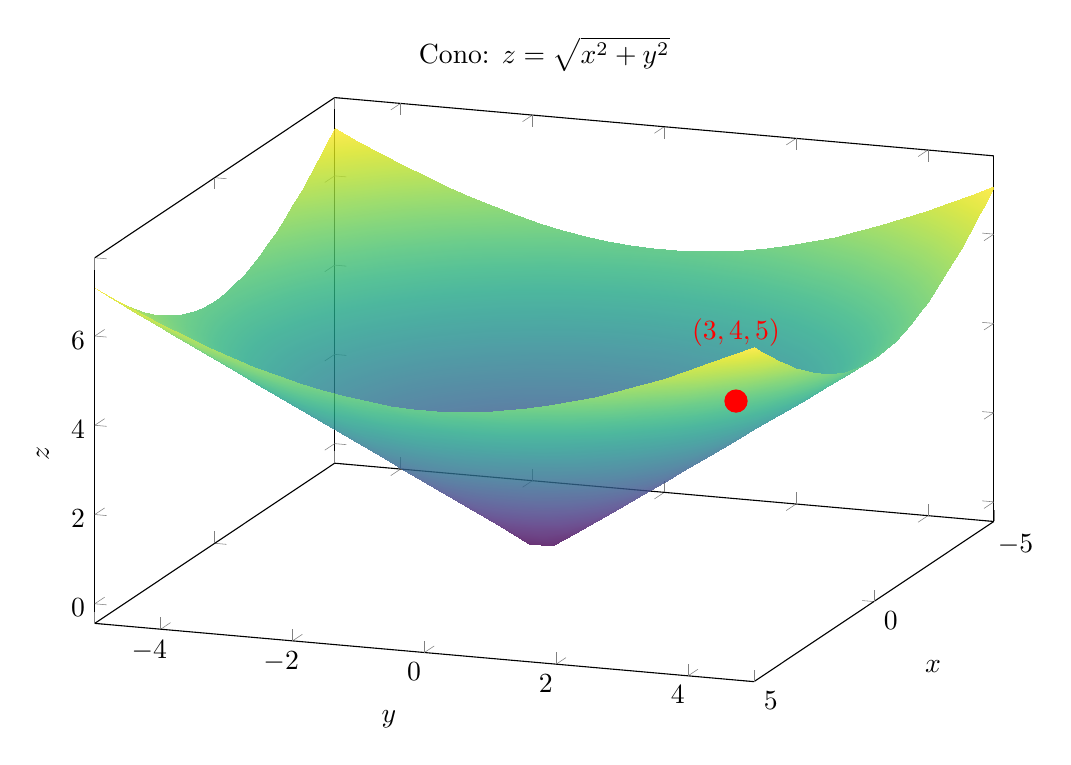
\begin{tikzpicture}
  \begin{axis}[
      view={110}{25},
      width=13cm, height=9cm,
      xlabel={$x$}, ylabel={$y$}, zlabel={$z$},
      domain=-5:5, y domain=-5:5,
      samples=30, samples y=30,
      colormap/viridis,
      title={Cono: \(z = \sqrt{x^2 + y^2}\)}
  ]
    % Superficie del cono
    \addplot3[surf,opacity=0.8,shader=interp] {sqrt(x^2 + y^2)};
    
    % Punto de interés (3,4,5)
    \addplot3[only marks, mark=*, mark size=4pt, color=red] coordinates {(3,4,5)};
    \node[anchor=south] at (axis cs:3,4,6) {\textcolor{red}{$(3,4,5)$}};
  \end{axis}
\end{tikzpicture}
\caption{Superficie cónica con punto de análisis en \((3,4,5)\).}
\label{fig:cono}
\end{figure}

\paragraph{Conclusión.}

La construcción geométrica de derivadas parciales nos permite:
\begin{itemize}
  \item \textbf{Visualizar} cómo una superficie cambia localmente en diferentes direcciones
  \item \textbf{Comprender} que cada derivada parcial es la pendiente de una curva específica
  \item \textbf{Utilizar software} para verificar y explorar cálculos analíticos
  \item \textbf{Desarrollar intuición} sobre el comportamiento de funciones multivariables
\end{itemize}

\subsubsection{Reglas de derivación parcial}

\begin{TemaBox}[Reglas de derivación: Extensión al caso multivariable]
Las reglas de derivación que conocemos del cálculo de una variable se extienden naturalmente a las derivadas parciales. La diferencia clave es que al derivar respecto a una variable, tratamos las demás como constantes.
\end{TemaBox}

\paragraph{Introducción.}
Las reglas de derivación parcial nos permiten calcular derivadas de funciones complejas de manera sistemática y eficiente. Estas reglas son idénticas a las del cálculo de una variable, pero aplicadas variable por variable.

\paragraph{Reglas básicas.}

Sea \(f(x,y)\) y \(g(x,y)\) funciones de dos variables, y \(c\) una constante.

\begin{InfoBox}
\Meta{Regla 1: Constante}{}
\[
\frac{\partial}{\partial x}(c) = 0, \quad \frac{\partial}{\partial y}(c) = 0
\]

\Meta{Regla 2: Constante por una función}{}
\[
\frac{\partial}{\partial x}[c \cdot f(x,y)] = c \cdot \frac{\partial f}{\partial x}
\]

\Meta{Regla 3: Suma y diferencia}{}
\[
\frac{\partial}{\partial x}[f(x,y) \pm g(x,y)] = \frac{\partial f}{\partial x} \pm \frac{\partial g}{\partial x}
\]

\Meta{Regla 4: Producto}{}
\[
\frac{\partial}{\partial x}[f(x,y) \cdot g(x,y)] = f \cdot \frac{\partial g}{\partial x} + g \cdot \frac{\partial f}{\partial x}
\]

\Meta{Regla 5: Cociente}{}
\[
\frac{\partial}{\partial x}\left[\frac{f(x,y)}{g(x,y)}\right] = \frac{g \cdot \frac{\partial f}{\partial x} - f \cdot \frac{\partial g}{\partial x}}{g^2}
\]

\Meta{Regla 6: Potencia}{}
\[
\frac{\partial}{\partial x}[f(x,y)]^n = n[f(x,y)]^{n-1} \cdot \frac{\partial f}{\partial x}
\]
\end{InfoBox}

\paragraph{Tabla resumen de derivadas parciales comunes.}

\begin{table}[h!]
\centering
\begin{tabular}{|c|c|c|}
\hline
\textbf{Función} & \(\boldsymbol{\frac{\partial f}{\partial x}}\) & \(\boldsymbol{\frac{\partial f}{\partial y}}\) \\
\hline
\(f(x,y) = x^n\) & \(nx^{n-1}\) & \(0\) \\
\hline
\(f(x,y) = y^n\) & \(0\) & \(ny^{n-1}\) \\
\hline
\(f(x,y) = x^n y^m\) & \(nx^{n-1}y^m\) & \(mx^n y^{m-1}\) \\
\hline
\(f(x,y) = e^x\) & \(e^x\) & \(0\) \\
\hline
\(f(x,y) = e^{xy}\) & \(ye^{xy}\) & \(xe^{xy}\) \\
\hline
\(f(x,y) = \ln(x)\) & \(\frac{1}{x}\) & \(0\) \\
\hline
\(f(x,y) = \ln(xy)\) & \(\frac{1}{x}\) & \(\frac{1}{y}\) \\
\hline
\(f(x,y) = \sin(x)\) & \(\cos(x)\) & \(0\) \\
\hline
\(f(x,y) = \sin(xy)\) & \(y\cos(xy)\) & \(x\cos(xy)\) \\
\hline
\(f(x,y) = \cos(x)\) & \(-\sin(x)\) & \(0\) \\
\hline
\(f(x,y) = \tan(x)\) & \(\sec^2(x)\) & \(0\) \\
\hline
\end{tabular}
\caption{Derivadas parciales de funciones comunes.}
\label{tab:derivadas_comunes}
\end{table}

\paragraph{Ejemplos resueltos detallados.}

\begin{EjercicioBox}[Ejemplo 1: Regla de la suma y producto]
Calcular las derivadas parciales de:
\[
f(x,y) = 3x^2y + 5xy^3 - 7x + 2y
\]

\textbf{Solución:}

\textbf{Para} \(\frac{\partial f}{\partial x}\): Derivamos término por término respecto a \(x\)

\begin{align*}
\frac{\partial f}{\partial x} &= \frac{\partial}{\partial x}(3x^2y) + \frac{\partial}{\partial x}(5xy^3) - \frac{\partial}{\partial x}(7x) + \frac{\partial}{\partial x}(2y) \\
&= 3y \cdot 2x + 5y^3 \cdot 1 - 7 + 0 \\
&= \boxed{6xy + 5y^3 - 7}
\end{align*}

\textbf{Para} \(\frac{\partial f}{\partial y}\): Derivamos término por término respecto a \(y\)

\begin{align*}
\frac{\partial f}{\partial y} &= \frac{\partial}{\partial y}(3x^2y) + \frac{\partial}{\partial y}(5xy^3) - \frac{\partial}{\partial y}(7x) + \frac{\partial}{\partial y}(2y) \\
&= 3x^2 \cdot 1 + 5x \cdot 3y^2 - 0 + 2 \\
&= \boxed{3x^2 + 15xy^2 + 2}
\end{align*}
\end{EjercicioBox}

\begin{EjercicioBox}[Ejemplo 2: Regla del producto]
Calcular las derivadas parciales de:
\[
f(x,y) = (x^2 + y)(3x - y^2)
\]

\textbf{Solución:}

\textbf{Para} \(\frac{\partial f}{\partial x}\): Usamos la regla del producto

Sean \(u = x^2 + y\) y \(v = 3x - y^2\)

\begin{align*}
\frac{\partial f}{\partial x} &= u \cdot \frac{\partial v}{\partial x} + v \cdot \frac{\partial u}{\partial x} \\
&= (x^2 + y) \cdot 3 + (3x - y^2) \cdot 2x \\
&= 3x^2 + 3y + 6x^2 - 2xy^2 \\
&= \boxed{9x^2 - 2xy^2 + 3y}
\end{align*}

\textbf{Para} \(\frac{\partial f}{\partial y}\):

\begin{align*}
\frac{\partial f}{\partial y} &= u \cdot \frac{\partial v}{\partial y} + v \cdot \frac{\partial u}{\partial y} \\
&= (x^2 + y) \cdot (-2y) + (3x - y^2) \cdot 1 \\
&= -2x^2y - 2y^2 + 3x - y^2 \\
&= \boxed{-2x^2y - 3y^2 + 3x}
\end{align*}
\end{EjercicioBox}

\begin{EjercicioBox}[Ejemplo 3: Regla del cociente]
Calcular las derivadas parciales de:
\[
f(x,y) = \frac{x^2 + y}{x - 2y}
\]

\textbf{Solución:}

Sean \(u = x^2 + y\) y \(v = x - 2y\)

\textbf{Para} \(\frac{\partial f}{\partial x}\): Aplicamos la regla del cociente

\begin{align*}
\frac{\partial f}{\partial x} &= \frac{v \cdot \frac{\partial u}{\partial x} - u \cdot \frac{\partial v}{\partial x}}{v^2} \\
&= \frac{(x - 2y) \cdot 2x - (x^2 + y) \cdot 1}{(x - 2y)^2} \\
&= \frac{2x^2 - 4xy - x^2 - y}{(x - 2y)^2} \\
&= \boxed{\frac{x^2 - 4xy - y}{(x - 2y)^2}}
\end{align*}

\textbf{Para} \(\frac{\partial f}{\partial y}\):

\begin{align*}
\frac{\partial f}{\partial y} &= \frac{v \cdot \frac{\partial u}{\partial y} - u \cdot \frac{\partial v}{\partial y}}{v^2} \\
&= \frac{(x - 2y) \cdot 1 - (x^2 + y) \cdot (-2)}{(x - 2y)^2} \\
&= \frac{x - 2y + 2x^2 + 2y}{(x - 2y)^2} \\
&= \boxed{\frac{2x^2 + x}{(x - 2y)^2}}
\end{align*}
\end{EjercicioBox}

\begin{EjercicioBox}[Ejemplo 4: Regla de la potencia (cadena)]
Calcular las derivadas parciales de:
\[
f(x,y) = (x^3 + xy^2)^5
\]

\textbf{Solución:}

Sea \(u = x^3 + xy^2\), entonces \(f = u^5\)

\textbf{Para} \(\frac{\partial f}{\partial x}\): Aplicamos la regla de la cadena

\begin{align*}
\frac{\partial f}{\partial x} &= 5u^4 \cdot \frac{\partial u}{\partial x} \\
&= 5(x^3 + xy^2)^4 \cdot (3x^2 + y^2) \\
&= \boxed{5(x^3 + xy^2)^4(3x^2 + y^2)}
\end{align*}

\textbf{Para} \(\frac{\partial f}{\partial y}\):

\begin{align*}
\frac{\partial f}{\partial y} &= 5u^4 \cdot \frac{\partial u}{\partial y} \\
&= 5(x^3 + xy^2)^4 \cdot (2xy) \\
&= \boxed{10xy(x^3 + xy^2)^4}
\end{align*}
\end{EjercicioBox}

\begin{EjercicioBox}[Ejemplo 5: Funciones exponenciales y trigonométricas]
Calcular las derivadas parciales de:
\[
f(x,y) = e^{x^2y} \sin(xy)
\]

\textbf{Solución:}

Usamos la regla del producto: \(f = e^{x^2y} \cdot \sin(xy)\)

\textbf{Para} \(\frac{\partial f}{\partial x}\):

\begin{align*}
\frac{\partial f}{\partial x} &= e^{x^2y} \cdot \frac{\partial}{\partial x}[\sin(xy)] + \sin(xy) \cdot \frac{\partial}{\partial x}[e^{x^2y}] \\
&= e^{x^2y} \cdot \cos(xy) \cdot y + \sin(xy) \cdot e^{x^2y} \cdot 2xy \\
&= e^{x^2y}[y\cos(xy) + 2xy\sin(xy)] \\
&= \boxed{ye^{x^2y}[\cos(xy) + 2x\sin(xy)]}
\end{align*}

\textbf{Para} \(\frac{\partial f}{\partial y}\):

\begin{align*}
\frac{\partial f}{\partial y} &= e^{x^2y} \cdot \frac{\partial}{\partial y}[\sin(xy)] + \sin(xy) \cdot \frac{\partial}{\partial y}[e^{x^2y}] \\
&= e^{x^2y} \cdot \cos(xy) \cdot x + \sin(xy) \cdot e^{x^2y} \cdot x^2 \\
&= xe^{x^2y}[\cos(xy) + x\sin(xy)] \\
&= \boxed{xe^{x^2y}[\cos(xy) + x\sin(xy)]}
\end{align*}
\end{EjercicioBox}

\begin{EjercicioBox}[Ejemplo 6: Función logarítmica]
Calcular las derivadas parciales de:
\[
f(x,y) = \ln(x^2 + y^2 + 1)
\]

\textbf{Solución:}

Sea \(u = x^2 + y^2 + 1\), entonces \(f = \ln(u)\)

\textbf{Para} \(\frac{\partial f}{\partial x}\): Usamos la regla de la cadena

\begin{align*}
\frac{\partial f}{\partial x} &= \frac{1}{u} \cdot \frac{\partial u}{\partial x} \\
&= \frac{1}{x^2 + y^2 + 1} \cdot 2x \\
&= \boxed{\frac{2x}{x^2 + y^2 + 1}}
\end{align*}

\textbf{Para} \(\frac{\partial f}{\partial y}\):

\begin{align*}
\frac{\partial f}{\partial y} &= \frac{1}{u} \cdot \frac{\partial u}{\partial y} \\
&= \frac{1}{x^2 + y^2 + 1} \cdot 2y \\
&= \boxed{\frac{2y}{x^2 + y^2 + 1}}
\end{align*}
\end{EjercicioBox}

\paragraph{Derivadas parciales de orden superior.}

Las derivadas parciales pueden derivarse nuevamente, obteniendo derivadas de segundo orden o superiores.

\begin{InfoBox}
\Meta{Notación}{Para \(f(x,y)\):}

\textbf{Segundas derivadas parciales:}
\begin{itemize}
  \item \(\frac{\partial^2 f}{\partial x^2} = f_{xx}\): derivar dos veces respecto a \(x\)
  \item \(\frac{\partial^2 f}{\partial y^2} = f_{yy}\): derivar dos veces respecto a \(y\)
  \item \(\frac{\partial^2 f}{\partial x \partial y} = f_{xy}\): derivar primero respecto a \(y\), luego respecto a \(x\)
  \item \(\frac{\partial^2 f}{\partial y \partial x} = f_{yx}\): derivar primero respecto a \(x\), luego respecto a \(y\)
\end{itemize}

\Meta{Teorema de Schwarz}{Si las derivadas parciales mixtas \(f_{xy}\) y \(f_{yx}\) son continuas, entonces:}
\[
\frac{\partial^2 f}{\partial x \partial y} = \frac{\partial^2 f}{\partial y \partial x}
\]
Es decir, el orden de derivación no importa.
\end{InfoBox}

\begin{EjercicioBox}[Ejemplo 7: Derivadas de segundo orden]
Calcular todas las segundas derivadas parciales de:
\[
f(x,y) = x^3y^2 + x^2y
\]

\textbf{Solución:}

\textbf{Primero calculamos las derivadas de primer orden:}
\begin{align*}
f_x &= 3x^2y^2 + 2xy \\
f_y &= 2x^3y + x^2
\end{align*}

\textbf{Ahora las segundas derivadas:}

\begin{align*}
f_{xx} &= \frac{\partial}{\partial x}(3x^2y^2 + 2xy) = \boxed{6xy^2 + 2y} \\[0.5em]
f_{yy} &= \frac{\partial}{\partial y}(2x^3y + x^2) = \boxed{2x^3} \\[0.5em]
f_{xy} &= \frac{\partial}{\partial y}(3x^2y^2 + 2xy) = \boxed{6x^2y + 2x} \\[0.5em]
f_{yx} &= \frac{\partial}{\partial x}(2x^3y + x^2) = \boxed{6x^2y + 2x}
\end{align*}

\textbf{Verificación:} Como esperábamos por el Teorema de Schwarz: \(f_{xy} = f_{yx}\)
\end{EjercicioBox}

\paragraph{Errores comunes al calcular derivadas parciales.}

\begin{itemize}
  \item \textbf{Error 1:} Olvidar que las otras variables son constantes.
  
  \textit{Incorrecto:} \(\frac{\partial}{\partial x}(xy^2) = y^2 + 2xy\)
  
  \textit{Correcto:} \(\frac{\partial}{\partial x}(xy^2) = y^2\) (porque \(y\) es constante)
  
  \item \textbf{Error 2:} Confundir el orden en derivadas mixtas.
  
  Para \(\frac{\partial^2 f}{\partial x \partial y}\): primero derivar respecto a \(y\), luego respecto a \(x\)
  
  \item \textbf{Error 3:} No aplicar la regla de la cadena cuando es necesaria.
  
  \textit{Incorrecto:} \(\frac{\partial}{\partial x}[\sin(x^2y)] = \cos(x^2y)\)
  
  \textit{Correcto:} \(\frac{\partial}{\partial x}[\sin(x^2y)] = \cos(x^2y) \cdot 2xy\)
\end{itemize}

\paragraph{Ejercicios propuestos.}

Calcular las derivadas parciales de las siguientes funciones:

\begin{enumerate}
  \item \(f(x,y) = 5x^4y^3 - 3x^2y + 7xy^2 - 2\)
  
  \item \(f(x,y) = \frac{x^3 - y^3}{x + y}\)
  
  \item \(f(x,y) = e^{x/y} + \ln(x^2 + y^2)\)
  
  \item \(f(x,y) = x^y\) \textit{(Sugerencia: \(x^y = e^{y\ln x}\))}
  
  \item \(f(x,y) = \cos(x^2 + y^2) \cdot e^{xy}\)
  
  \item \(f(x,y,z) = xyz + x^2y + y^2z + z^2x\) (tres variables)
  
  \item Calcular \(f_{xx}\), \(f_{yy}\), \(f_{xy}\) para \(f(x,y) = \sin(x)\cos(y)\)
  
  \item Verificar que \(f_{xy} = f_{yx}\) para \(f(x,y) = e^{xy^2}\)
\end{enumerate}

\subsubsection{Regla de la cadena para varias variables}

\begin{TemaBox}[Regla de la cadena: Composición de funciones multivariables]
La regla de la cadena para funciones de varias variables nos permite calcular derivadas cuando las variables son, a su vez, funciones de otras variables. Es una extensión natural de la regla de la cadena del cálculo de una variable y es fundamental en física, ingeniería y optimización.
\end{TemaBox}

\paragraph{Introducción.}
En cálculo de una variable, la regla de la cadena establece que si \(y = f(u)\) y \(u = g(x)\), entonces:
\[
\frac{dy}{dx} = \frac{dy}{du} \cdot \frac{du}{dx}
\]

Para funciones de varias variables, esta regla se extiende considerando todas las trayectorias de dependencia entre variables.

\paragraph{Caso 1: Función de dos variables con dependencia de una sola variable.}

\begin{InfoBox}
\Meta{Teorema (Regla de la cadena - Caso 1)}{Sea \(z = f(x,y)\) una función diferenciable de \(x\) e \(y\), donde:}
\begin{itemize}
  \item \(x = x(t)\)
  \item \(y = y(t)\)
\end{itemize}

Entonces la \textbf{derivada total} de \(z\) respecto a \(t\) es:
\[
\frac{dz}{dt} = \frac{\partial z}{\partial x} \cdot \frac{dx}{dt} + \frac{\partial z}{\partial y} \cdot \frac{dy}{dt}
\]

\Meta{Interpretación}{La tasa de cambio de \(z\) respecto a \(t\) se obtiene sumando las contribuciones de cada variable intermedia.}
\end{InfoBox}

\paragraph{Visualización de las dependencias.}

Para visualizar la regla de la cadena, imaginamos un diagrama de árbol con las siguientes dependencias:

\begin{InfoBox}
\Meta{Caminos de dependencia}{Existen dos caminos desde \(t\) hasta \(z\):}
\begin{itemize}
  \item \textbf{Camino 1:} \(t \to x \to z\) contribuye: \(\frac{\partial z}{\partial x} \cdot \frac{dx}{dt}\)
  \item \textbf{Camino 2:} \(t \to y \to z\) contribuye: \(\frac{\partial z}{\partial y} \cdot \frac{dy}{dt}\)
\end{itemize}

La derivada total es la suma de las contribuciones de ambos caminos.
\end{InfoBox}

\begin{EjercicioBox}[Ejemplo 1: Caso básico]
Sea \(z = x^2 + xy + y^2\) donde \(x = t^2\) y \(y = t^3\). Calcular \(\frac{dz}{dt}\).

\textbf{Solución:}

\textbf{Método 1: Aplicando la regla de la cadena}

Primero calculamos las derivadas parciales de \(z\):
\begin{align*}
\frac{\partial z}{\partial x} &= 2x + y \\
\frac{\partial z}{\partial y} &= x + 2y
\end{align*}

Luego las derivadas de \(x\) e \(y\) respecto a \(t\):
\begin{align*}
\frac{dx}{dt} &= 2t \\
\frac{dy}{dt} &= 3t^2
\end{align*}

Aplicamos la regla de la cadena:
\begin{align*}
\frac{dz}{dt} &= \frac{\partial z}{\partial x} \cdot \frac{dx}{dt} + \frac{\partial z}{\partial y} \cdot \frac{dy}{dt} \\
&= (2x + y)(2t) + (x + 2y)(3t^2) \\
&= (2t^2 + t^3)(2t) + (t^2 + 2t^3)(3t^2) \\
&= 4t^3 + 2t^4 + 3t^4 + 6t^5 \\
&= \boxed{6t^5 + 5t^4 + 4t^3}
\end{align*}

\textbf{Método 2: Sustitución directa (verificación)}

Sustituimos \(x = t^2\) y \(y = t^3\) en \(z\):
\begin{align*}
z &= (t^2)^2 + (t^2)(t^3) + (t^3)^2 \\
&= t^4 + t^5 + t^6
\end{align*}

Derivamos directamente:
\[
\frac{dz}{dt} = 4t^3 + 5t^4 + 6t^5 = \boxed{6t^5 + 5t^4 + 4t^3}
\]

\textbf{Ambos métodos dan el mismo resultado.}
\end{EjercicioBox}

\begin{EjercicioBox}[Ejemplo 2: Funciones trigonométricas]
Sea \(z = e^x \sin(y)\) donde \(x = t^2\) y \(y = \pi t\). Calcular \(\frac{dz}{dt}\) cuando \(t = 1\).

\textbf{Solución:}

Calculamos las derivadas parciales:
\begin{align*}
\frac{\partial z}{\partial x} &= e^x \sin(y) \\
\frac{\partial z}{\partial y} &= e^x \cos(y)
\end{align*}

Las derivadas respecto a \(t\):
\begin{align*}
\frac{dx}{dt} &= 2t \\
\frac{dy}{dt} &= \pi
\end{align*}

Aplicamos la regla de la cadena:
\begin{align*}
\frac{dz}{dt} &= e^x \sin(y) \cdot 2t + e^x \cos(y) \cdot \pi \\
&= e^{t^2}[\sin(\pi t) \cdot 2t + \cos(\pi t) \cdot \pi]
\end{align*}

Evaluamos en \(t = 1\):
\begin{align*}
\frac{dz}{dt}\bigg|_{t=1} &= e^{1}[\sin(\pi) \cdot 2 + \cos(\pi) \cdot \pi] \\
&= e[0 \cdot 2 + (-1) \cdot \pi] \\
&= \boxed{-\pi e}
\end{align*}
\end{EjercicioBox}

\paragraph{Caso 2: Función de dos variables con dependencia de dos variables.}

\begin{InfoBox}
\Meta{Teorema (Regla de la cadena - Caso 2)}{Sea \(z = f(x,y)\) donde:}
\begin{itemize}
  \item \(x = x(u,v)\)
  \item \(y = y(u,v)\)
\end{itemize}

Entonces:
\[
\frac{\partial z}{\partial u} = \frac{\partial z}{\partial x} \cdot \frac{\partial x}{\partial u} + \frac{\partial z}{\partial y} \cdot \frac{\partial y}{\partial u}
\]

\[
\frac{\partial z}{\partial v} = \frac{\partial z}{\partial x} \cdot \frac{\partial x}{\partial v} + \frac{\partial z}{\partial y} \cdot \frac{\partial y}{\partial v}
\]
\end{InfoBox}

\paragraph{Visualización para el Caso 2.}

Para este caso más complejo, existen cuatro caminos desde las variables \(u\) y \(v\) hasta \(z\):

\begin{InfoBox}
\Meta{Caminos de dependencia para el Caso 2}{Cuatro caminos:}
\begin{itemize}
  \item \textbf{Camino 1:} \(u \to x \to z\) contribuye: \(\frac{\partial z}{\partial x} \cdot \frac{\partial x}{\partial u}\)
  \item \textbf{Camino 2:} \(u \to y \to z\) contribuye: \(\frac{\partial z}{\partial y} \cdot \frac{\partial y}{\partial u}\)
  \item \textbf{Camino 3:} \(v \to x \to z\) contribuye: \(\frac{\partial z}{\partial x} \cdot \frac{\partial x}{\partial v}\)
  \item \textbf{Camino 4:} \(v \to y \to z\) contribuye: \(\frac{\partial z}{\partial y} \cdot \frac{\partial y}{\partial v}\)
\end{itemize}

Por tanto:
\begin{align*}
\frac{\partial z}{\partial u} &= \frac{\partial z}{\partial x}\frac{\partial x}{\partial u} + \frac{\partial z}{\partial y}\frac{\partial y}{\partial u} \\
\frac{\partial z}{\partial v} &= \frac{\partial z}{\partial x}\frac{\partial x}{\partial v} + \frac{\partial z}{\partial y}\frac{\partial y}{\partial v}
\end{align*}
\end{InfoBox}

\begin{EjercicioBox}[Ejemplo 3: Coordenadas polares]
Sea \(z = x^2 + y^2\) donde \(x = r\cos(\theta)\) y \(y = r\sin(\theta)\). Calcular \(\frac{\partial z}{\partial r}\) y \(\frac{\partial z}{\partial \theta}\).

\textbf{Solución:}

Calculamos las derivadas parciales de \(z\):
\begin{align*}
\frac{\partial z}{\partial x} &= 2x \\
\frac{\partial z}{\partial y} &= 2y
\end{align*}

Las derivadas de \(x\) e \(y\) respecto a \(r\) y \(\theta\):
\begin{align*}
\frac{\partial x}{\partial r} &= \cos(\theta), \quad \frac{\partial x}{\partial \theta} = -r\sin(\theta) \\
\frac{\partial y}{\partial r} &= \sin(\theta), \quad \frac{\partial y}{\partial \theta} = r\cos(\theta)
\end{align*}

\textbf{Para} \(\frac{\partial z}{\partial r}\):
\begin{align*}
\frac{\partial z}{\partial r} &= \frac{\partial z}{\partial x} \cdot \frac{\partial x}{\partial r} + \frac{\partial z}{\partial y} \cdot \frac{\partial y}{\partial r} \\
&= 2x \cdot \cos(\theta) + 2y \cdot \sin(\theta) \\
&= 2r\cos^2(\theta) + 2r\sin^2(\theta) \\
&= 2r(\cos^2(\theta) + \sin^2(\theta)) \\
&= \boxed{2r}
\end{align*}

\textbf{Para} \(\frac{\partial z}{\partial \theta}\):
\begin{align*}
\frac{\partial z}{\partial \theta} &= \frac{\partial z}{\partial x} \cdot \frac{\partial x}{\partial \theta} + \frac{\partial z}{\partial y} \cdot \frac{\partial y}{\partial \theta} \\
&= 2x \cdot (-r\sin(\theta)) + 2y \cdot r\cos(\theta) \\
&= -2r^2\cos(\theta)\sin(\theta) + 2r^2\sin(\theta)\cos(\theta) \\
&= \boxed{0}
\end{align*}

\textbf{Interpretación:} \(\frac{\partial z}{\partial r} = 2r\) indica que \(z\) crece linealmente con \(r\). \(\frac{\partial z}{\partial \theta} = 0\) confirma que \(z = x^2 + y^2\) no depende del ángulo (es simétrica circularmente).
\end{EjercicioBox}

\begin{EjercicioBox}[Ejemplo 4: Caso general]
Sea \(z = x^2y + xy^2\) donde \(x = uv\) y \(y = u - v\). Calcular \(\frac{\partial z}{\partial u}\) y \(\frac{\partial z}{\partial v}\).

\textbf{Solución:}

Derivadas parciales de \(z\):
\begin{align*}
\frac{\partial z}{\partial x} &= 2xy + y^2 \\
\frac{\partial z}{\partial y} &= x^2 + 2xy
\end{align*}

Derivadas de \(x\) e \(y\):
\begin{align*}
\frac{\partial x}{\partial u} &= v, \quad \frac{\partial x}{\partial v} = u \\
\frac{\partial y}{\partial u} &= 1, \quad \frac{\partial y}{\partial v} = -1
\end{align*}

\textbf{Para} \(\frac{\partial z}{\partial u}\):
\begin{align*}
\frac{\partial z}{\partial u} &= (2xy + y^2) \cdot v + (x^2 + 2xy) \cdot 1 \\
&= v(2xy + y^2) + x^2 + 2xy
\end{align*}

Sustituyendo \(x = uv\) y \(y = u - v\):
\begin{align*}
\frac{\partial z}{\partial u} &= v[2uv(u-v) + (u-v)^2] + (uv)^2 + 2uv(u-v) \\
&= 2u v^2(u-v) + v(u-v)^2 + u^2v^2 + 2uv(u-v) \\
&= \boxed{2u^2v^2 - 2uv^3 + u^2v - 2uv^2 + v^3 + u^2v^2 + 2u^2v - 2uv^2}
\end{align*}

Simplificando:
\[
\frac{\partial z}{\partial u} = \boxed{3u^2v^2 + 2u^2v + u^2v - 4uv^2 + v^3}
\]

\textbf{Para} \(\frac{\partial z}{\partial v}\):
\begin{align*}
\frac{\partial z}{\partial v} &= (2xy + y^2) \cdot u + (x^2 + 2xy) \cdot (-1) \\
&= u(2xy + y^2) - x^2 - 2xy
\end{align*}

(Se puede desarrollar de manera similar sustituyendo valores)
\end{EjercicioBox}

\paragraph{Caso 3: Derivada implícita.}

Cuando tenemos una ecuación implícita \(F(x,y) = 0\), podemos usar la regla de la cadena para encontrar \(\frac{dy}{dx}\).

\begin{InfoBox}
\Meta{Derivación implícita}{Para \(F(x,y) = 0\):}
\[
\frac{dy}{dx} = -\frac{\frac{\partial F}{\partial x}}{\frac{\partial F}{\partial y}}
\]

\Meta{Generalización}{Para \(F(x,y,z) = 0\):}
\[
\frac{\partial z}{\partial x} = -\frac{\frac{\partial F}{\partial x}}{\frac{\partial F}{\partial z}}, \quad
\frac{\partial z}{\partial y} = -\frac{\frac{\partial F}{\partial y}}{\frac{\partial F}{\partial z}}
\]
\end{InfoBox}

\begin{EjercicioBox}[Ejemplo 5: Derivación implícita]
Para la ecuación \(x^3 + y^3 + xyz = 10\), calcular \(\frac{\partial z}{\partial x}\) y \(\frac{\partial z}{\partial y}\).

\textbf{Solución:}

Sea \(F(x,y,z) = x^3 + y^3 + xyz - 10\)

Calculamos las derivadas parciales de \(F\):
\begin{align*}
\frac{\partial F}{\partial x} &= 3x^2 + yz \\
\frac{\partial F}{\partial y} &= 3y^2 + xz \\
\frac{\partial F}{\partial z} &= xy
\end{align*}

Aplicamos la fórmula:
\[
\frac{\partial z}{\partial x} = -\frac{3x^2 + yz}{xy} = \boxed{-\frac{3x^2 + yz}{xy}}
\]

\[
\frac{\partial z}{\partial y} = -\frac{3y^2 + xz}{xy} = \boxed{-\frac{3y^2 + xz}{xy}}
\]
\end{EjercicioBox}

\paragraph{Aplicaciones prácticas.}

\begin{enumerate}
  \item \textbf{Física:} Cambio de coordenadas (cartesianas a polares, cilíndricas, esféricas)
  \item \textbf{Termodinámica:} Relaciones entre variables de estado
  \item \textbf{Optimización:} Funciones objetivo con restricciones paramétricas
  \item \textbf{Ingeniería:} Análisis de sensibilidad en sistemas complejos
  \item \textbf{Cinemática:} Velocidad y aceleración en trayectorias curvas
\end{enumerate}

\paragraph{Ejercicios propuestos.}

\begin{enumerate}
  \item Sea \(z = x^2 - y^2\) donde \(x = e^t\) y \(y = e^{-t}\). Calcular \(\frac{dz}{dt}\).
  
  \item Sea \(w = xyz\) donde \(x = t\), \(y = t^2\), \(z = t^3\). Calcular \(\frac{dw}{dt}\) cuando \(t = 2\).
  
  \item Sea \(z = \ln(x^2 + y^2)\) donde \(x = r\cos(\theta)\) y \(y = r\sin(\theta)\). Calcular \(\frac{\partial z}{\partial r}\) y \(\frac{\partial z}{\partial \theta}\).
  
  \item Sea \(z = e^{x+y}\) donde \(x = u^2 - v^2\) y \(y = 2uv\). Calcular \(\frac{\partial z}{\partial u}\) y \(\frac{\partial z}{\partial v}\).
  
  \item Para la ecuación implícita \(x^2 + y^2 + z^2 = 25\), calcular \(\frac{\partial z}{\partial x}\) y \(\frac{\partial z}{\partial y}\).
  
  \item Sea \(w = f(x,y,z)\) donde \(x = r\sin(\phi)\cos(\theta)\), \(y = r\sin(\phi)\sin(\theta)\), \(z = r\cos(\phi)\) (coordenadas esféricas). Expresar \(\frac{\partial w}{\partial r}\) usando la regla de la cadena.
  
  \item Verificar que si \(z = f(x-y, y-x)\), entonces \(\frac{\partial z}{\partial x} + \frac{\partial z}{\partial y} = 0\).
\end{enumerate}

\paragraph{Resumen de la regla de la cadena.}

\begin{table}[h!]
\centering
\begin{tabular}{|l|l|}
\hline
\textbf{Caso} & \textbf{Fórmula} \\
\hline
\(z = f(x,y)\), \(x=x(t)\), \(y=y(t)\) & \(\displaystyle \frac{dz}{dt} = \frac{\partial z}{\partial x}\frac{dx}{dt} + \frac{\partial z}{\partial y}\frac{dy}{dt}\) \\
\hline
\(z = f(x,y)\), \(x=x(u,v)\), \(y=y(u,v)\) & \(\displaystyle \frac{\partial z}{\partial u} = \frac{\partial z}{\partial x}\frac{\partial x}{\partial u} + \frac{\partial z}{\partial y}\frac{\partial y}{\partial u}\) \\
\hline
\(F(x,y,z) = 0\) & \(\displaystyle \frac{\partial z}{\partial x} = -\frac{\partial F/\partial x}{\partial F/\partial z}\) \\
\hline
\end{tabular}
\caption{Resumen de casos de la regla de la cadena.}
\label{tab:regla_cadena}
\end{table}

\subsection{Vector gradiente y derivada direccional}

\begin{TemaBox}[Vector gradiente y derivada direccional: Concepto unificador]
El gradiente es uno de los conceptos más importantes del cálculo multivariable. Unifica todas las derivadas parciales en un solo vector que apunta en la dirección de máximo crecimiento de la función. La derivada direccional nos permite medir la tasa de cambio en cualquier dirección deseada.
\end{TemaBox}

\paragraph{Introducción y contextualización.}

Hasta ahora hemos estudiado las derivadas parciales \(\frac{\partial f}{\partial x}\) y \(\frac{\partial f}{\partial y}\), que miden cómo cambia la función cuando nos movemos en las direcciones de los ejes coordenados. Pero, ¿qué sucede si queremos saber cómo cambia la función cuando nos movemos en cualquier otra dirección?

Imagina que estás de excursión en una montaña y tienes un mapa topográfico con curvas de nivel. Las derivadas parciales te dicen qué tan empinado es el terreno si caminas exactamente hacia el norte (\(y\)) o hacia el este (\(x\)). Pero si quieres caminar en dirección noreste, o en cualquier otra dirección, necesitas un concepto más general: \textbf{la derivada direccional}.

Además, si quieres encontrar la dirección más empinada para subir (o bajar) lo más rápido posible, necesitas el \textbf{vector gradiente}, que siempre apunta en la dirección de máxima pendiente ascendente.

\subsubsection{Cálculo e interpretación geométrica del gradiente y derivada direccional}

\paragraph{Definición: Vector gradiente.}

\begin{InfoBox}
\Meta{Definición}{Sea \(f(x,y)\) una función diferenciable. El \textbf{gradiente} de \(f\) se denota \(\nabla f\) (se lee "nabla \(f\)") y se define como:}
\[
\nabla f(x,y) = \left\langle \frac{\partial f}{\partial x}, \frac{\partial f}{\partial y} \right\rangle = \frac{\partial f}{\partial x}\mathbf{i} + \frac{\partial f}{\partial y}\mathbf{j}
\]

\Meta{Para funciones de tres variables}{\(f(x,y,z)\):}
\[
\nabla f(x,y,z) = \left\langle \frac{\partial f}{\partial x}, \frac{\partial f}{\partial y}, \frac{\partial f}{\partial z} \right\rangle
\]

\Meta{Notación alternativa}{También se escribe como \(\text{grad}\,f\).}
\end{InfoBox}

El gradiente es un \textbf{campo vectorial}: en cada punto \((x,y)\) del dominio de \(f\), el gradiente \(\nabla f(x,y)\) es un vector.

\paragraph{Propiedades geométricas del gradiente.}

El vector gradiente tiene propiedades geométricas fundamentales:

\begin{enumerate}
  \item \textbf{Dirección:} \(\nabla f\) apunta en la dirección de máximo crecimiento de \(f\).
  
  \item \textbf{Magnitud:} \(\|\nabla f\|\) es la razón de cambio máxima de \(f\) en ese punto.
  
  \item \textbf{Perpendicularidad:} \(\nabla f\) es perpendicular a las curvas de nivel de \(f\).
  
  \item \textbf{Cero en puntos críticos:} Si \(\nabla f = \mathbf{0}\), entonces \((x,y)\) es un punto crítico.
\end{enumerate}

\begin{EjercicioBox}[Ejemplo 1: Cálculo del gradiente]
Calcular el gradiente de \(f(x,y) = x^2 + xy + y^2\) y evaluarlo en el punto \((1,2)\).

\textbf{Solución:}

Calculamos las derivadas parciales:
\begin{align*}
\frac{\partial f}{\partial x} &= 2x + y \\
\frac{\partial f}{\partial y} &= x + 2y
\end{align*}

Por lo tanto, el gradiente es:
\[
\nabla f(x,y) = \langle 2x + y, x + 2y \rangle
\]

Evaluamos en \((1,2)\):
\[
\nabla f(1,2) = \langle 2(1) + 2, 1 + 2(2) \rangle = \langle 4, 5 \rangle
\]

\textbf{Interpretación:} En el punto \((1,2)\), la función crece más rápidamente en la dirección del vector \(\langle 4, 5 \rangle\), con una razón de cambio de \(\|\langle 4, 5 \rangle\| = \sqrt{16+25} = \sqrt{41} \approx 6.40\).
\end{EjercicioBox}

\begin{EjercicioBox}[Ejemplo 2: Gradiente de función exponencial]
Calcular \(\nabla f\) para \(f(x,y) = e^{x^2+y^2}\) en el punto \((0,0)\).

\textbf{Solución:}

\begin{align*}
\frac{\partial f}{\partial x} &= e^{x^2+y^2} \cdot 2x = 2xe^{x^2+y^2} \\
\frac{\partial f}{\partial y} &= e^{x^2+y^2} \cdot 2y = 2ye^{x^2+y^2}
\end{align*}

Por lo tanto:
\[
\nabla f(x,y) = \langle 2xe^{x^2+y^2}, 2ye^{x^2+y^2} \rangle
\]

En \((0,0)\):
\[
\nabla f(0,0) = \langle 2(0)e^{0}, 2(0)e^{0} \rangle = \langle 0, 0 \rangle
\]

\textbf{Interpretación:} El punto \((0,0)\) es un punto crítico (en este caso, un mínimo local).
\end{EjercicioBox}

\paragraph{Definición: Derivada direccional.}

Las derivadas parciales miden el cambio de \(f\) en las direcciones de los ejes. La derivada direccional generaliza esto a cualquier dirección.

\begin{InfoBox}
\Meta{Definición}{Sea \(f(x,y)\) una función diferenciable y \(\mathbf{u} = \langle a, b \rangle\) un \textbf{vector unitario} (es decir, \(\|\mathbf{u}\| = 1\)). La \textbf{derivada direccional} de \(f\) en la dirección de \(\mathbf{u}\) se denota \(D_{\mathbf{u}}f\) y se define como:}
\[
D_{\mathbf{u}}f(x,y) = \lim_{h \to 0} \frac{f(x + ha, y + hb) - f(x,y)}{h}
\]

\Meta{Fórmula práctica}{Si \(f\) es diferenciable:}
\[
D_{\mathbf{u}}f(x,y) = \nabla f(x,y) \cdot \mathbf{u} = \frac{\partial f}{\partial x}a + \frac{\partial f}{\partial y}b
\]

Esta fórmula nos dice que la derivada direccional es el producto punto entre el gradiente y el vector de dirección.
\end{InfoBox}

\paragraph{Relación entre gradiente y derivada direccional.}

La relación entre el gradiente y la derivada direccional es fundamental:

\begin{InfoBox}
\Meta{Teorema}{Sea \(f\) diferenciable y \(\mathbf{u}\) un vector unitario. Entonces:}
\[
D_{\mathbf{u}}f = \nabla f \cdot \mathbf{u} = \|\nabla f\| \|\mathbf{u}\| \cos(\theta) = \|\nabla f\| \cos(\theta)
\]
donde \(\theta\) es el ángulo entre \(\nabla f\) y \(\mathbf{u}\).

\Meta{Consecuencias importantes}{}
\begin{itemize}
  \item \textbf{Máximo:} \(D_{\mathbf{u}}f\) es máxima cuando \(\theta = 0\), es decir, cuando \(\mathbf{u}\) apunta en la dirección de \(\nabla f\). El valor máximo es \(\|\nabla f\|\).
  
  \item \textbf{Mínimo:} \(D_{\mathbf{u}}f\) es mínima cuando \(\theta = \pi\), es decir, cuando \(\mathbf{u}\) apunta en dirección opuesta a \(\nabla f\). El valor mínimo es \(-\|\nabla f\|\).
  
  \item \textbf{Cero:} \(D_{\mathbf{u}}f = 0\) cuando \(\theta = \pi/2\), es decir, cuando \(\mathbf{u}\) es perpendicular a \(\nabla f\). Esto ocurre en la dirección tangente a la curva de nivel.
\end{itemize}
\end{InfoBox}

\begin{EjercicioBox}[Ejemplo 3: Derivada direccional básica]
Sea \(f(x,y) = x^2 + y^2\). Calcular la derivada direccional en el punto \((3,4)\) en la dirección del vector \(\mathbf{v} = \langle 1, 1 \rangle\).

\textbf{Solución:}

\textbf{Paso 1:} Calcular el gradiente:
\begin{align*}
\frac{\partial f}{\partial x} &= 2x \\
\frac{\partial f}{\partial y} &= 2y
\end{align*}
\[
\nabla f(3,4) = \langle 2(3), 2(4) \rangle = \langle 6, 8 \rangle
\]

\textbf{Paso 2:} Normalizar el vector de dirección:
\[
\|\mathbf{v}\| = \sqrt{1^2 + 1^2} = \sqrt{2}
\]
\[
\mathbf{u} = \frac{\mathbf{v}}{\|\mathbf{v}\|} = \left\langle \frac{1}{\sqrt{2}}, \frac{1}{\sqrt{2}} \right\rangle
\]

\textbf{Paso 3:} Calcular la derivada direccional:
\begin{align*}
D_{\mathbf{u}}f(3,4) &= \nabla f(3,4) \cdot \mathbf{u} \\
&= \langle 6, 8 \rangle \cdot \left\langle \frac{1}{\sqrt{2}}, \frac{1}{\sqrt{2}} \right\rangle \\
&= \frac{6}{\sqrt{2}} + \frac{8}{\sqrt{2}} \\
&= \frac{14}{\sqrt{2}} = 7\sqrt{2} \approx \boxed{9.90}
\end{align*}

\textbf{Interpretación:} Si nos movemos desde \((3,4)\) en dirección \(45°\) (noreste), la función aumenta a una razón de aproximadamente \(9.90\) unidades por unidad de distancia.
\end{EjercicioBox}

\begin{EjercicioBox}[Ejemplo 4: Dirección de máximo crecimiento]
Para \(f(x,y) = x^2 - xy + y^2\) en el punto \((2,1)\):
\begin{enumerate}
  \item Encontrar la dirección de máximo crecimiento.
  \item Calcular la razón de cambio máxima.
  \item Encontrar la dirección de máximo decrecimiento.
\end{enumerate}

\textbf{Solución:}

\textbf{Calculamos el gradiente:}
\begin{align*}
\frac{\partial f}{\partial x} &= 2x - y \\
\frac{\partial f}{\partial y} &= -x + 2y
\end{align*}
\[
\nabla f(2,1) = \langle 2(2) - 1, -2 + 2(1) \rangle = \langle 3, 0 \rangle
\]

\textbf{a) Dirección de máximo crecimiento:}

El vector gradiente apunta en la dirección de máximo crecimiento. El vector unitario correspondiente es:
\[
\mathbf{u}_{\text{max}} = \frac{\nabla f}{\|\nabla f\|} = \frac{\langle 3, 0 \rangle}{3} = \boxed{\langle 1, 0 \rangle}
\]

La dirección es horizontal hacia la derecha (dirección positiva del eje \(x\)).

\textbf{b) Razón de cambio máxima:}
\[
\text{Razón máxima} = \|\nabla f(2,1)\| = \sqrt{3^2 + 0^2} = \boxed{3}
\]

\textbf{c) Dirección de máximo decrecimiento:}

Es la dirección opuesta al gradiente:
\[
\mathbf{u}_{\text{min}} = -\frac{\nabla f}{\|\nabla f\|} = \boxed{\langle -1, 0 \rangle}
\]

La razón de decrecimiento es \(-3\).
\end{EjercicioBox}

\begin{EjercicioBox}[Ejemplo 5: Temperatura y flujo de calor]
La temperatura en una placa metálica está dada por:
\[
T(x,y) = 100 - x^2 - 2y^2
\]
donde \(T\) se mide en grados Celsius y \(x, y\) en metros.

\begin{enumerate}
  \item Encontrar la dirección de máximo incremento de temperatura en el punto \((2,1)\).
  \item ¿Cuál es la razón de cambio máxima en ese punto?
  \item En qué dirección no cambia la temperatura (curva isotérmica)?
\end{enumerate}

\textbf{Solución:}

\textbf{Calculamos el gradiente:}
\begin{align*}
\frac{\partial T}{\partial x} &= -2x \\
\frac{\partial T}{\partial y} &= -4y
\end{align*}
\[
\nabla T(2,1) = \langle -2(2), -4(1) \rangle = \langle -4, -4 \rangle
\]

\textbf{a) Dirección de máximo incremento:}
\[
\mathbf{u}_{\text{max}} = \frac{\langle -4, -4 \rangle}{\sqrt{16+16}} = \frac{\langle -4, -4 \rangle}{4\sqrt{2}} = \left\langle \frac{-1}{\sqrt{2}}, \frac{-1}{\sqrt{2}} \right\rangle
\]

Esta dirección apunta hacia el suroeste (\(225°\)).

\textbf{b) Razón de cambio máxima:}
\[
\|\nabla T(2,1)\| = \sqrt{16+16} = 4\sqrt{2} \approx \boxed{5.66 \text{ °C/m}}
\]

\textbf{c) Dirección sin cambio:}

La temperatura no cambia en direcciones perpendiculares al gradiente. Si \(\nabla T = \langle -4, -4 \rangle\), las direcciones perpendiculares son:
\[
\mathbf{u}_{\perp} = \pm\left\langle \frac{1}{\sqrt{2}}, \frac{-1}{\sqrt{2}} \right\rangle
\]

Estas direcciones son tangentes a la curva isotérmica (curva de nivel de temperatura constante).
\end{EjercicioBox}

\paragraph{Interpretación física y geométrica.}

\begin{InfoBox}
\Meta{Interpretaciones del gradiente}{}

\textbf{1. Geométrica:}
\begin{itemize}
  \item El gradiente es perpendicular a las curvas de nivel.
  \item Apunta "cuesta arriba" en la superficie \(z = f(x,y)\).
  \item Su magnitud indica qué tan empinada es la superficie.
\end{itemize}

\textbf{2. Física (campo de temperaturas):}
\begin{itemize}
  \item \(\nabla T\) apunta en la dirección del flujo de calor.
  \item \(\|\nabla T\|\) indica la intensidad del gradiente térmico.
  \item El calor fluye de regiones calientes a frías.
\end{itemize}

\textbf{3. Optimización:}
\begin{itemize}
  \item Para maximizar \(f\), seguir la dirección de \(\nabla f\).
  \item Para minimizar \(f\), seguir la dirección de \(-\nabla f\).
  \item Este principio es la base del algoritmo de \textbf{gradiente descendente} en machine learning.
\end{itemize}
\end{InfoBox}

\paragraph{Aplicaciones prácticas.}

\begin{enumerate}
  \item \textbf{Física:} 
  \begin{itemize}
    \item Campos conservativos: \(\mathbf{F} = -\nabla U\) (fuerza desde potencial)
    \item Ley de Fourier: flujo de calor proporcional a \(-\nabla T\)
    \item Ley de Fick: difusión proporcional a \(-\nabla C\) (concentración)
  \end{itemize}
  
  \item \textbf{Ingeniería:}
  \begin{itemize}
    \item Optimización de diseños estructurales
    \item Control de procesos industriales
    \item Análisis de distribución de esfuerzos
  \end{itemize}
  
  \item \textbf{Machine Learning:}
  \begin{itemize}
    \item Gradiente descendente para entrenar redes neuronales
    \item Minimización de funciones de pérdida
    \item Backpropagation (propagación hacia atrás)
  \end{itemize}
  
  \item \textbf{Geografía y topografía:}
  \begin{itemize}
    \item Determinación de pendientes máximas
    \item Análisis de escorrentía de agua
    \item Planificación de rutas
  \end{itemize}
  
  \item \textbf{Economía:}
  \begin{itemize}
    \item Dirección de máximo beneficio
    \item Análisis marginal multivariable
    \item Optimización de portafolios
  \end{itemize}
\end{enumerate}

\paragraph{Ejercicios propuestos.}

\begin{enumerate}
  \item Calcular \(\nabla f\) para las siguientes funciones:
  \begin{enumerate}
    \item \(f(x,y) = \sin(x) + \cos(y)\)
    \item \(f(x,y) = \ln(x^2 + y^2)\)
    \item \(f(x,y,z) = xyz + x^2 + y^2 + z^2\)
  \end{enumerate}
  
  \item Para \(f(x,y) = x^3 - 3xy + y^3\), encontrar:
  \begin{enumerate}
    \item El gradiente en \((1,1)\)
    \item La dirección de máximo crecimiento en ese punto
    \item La razón de cambio máxima
  \end{enumerate}
  
  \item Calcular \(D_{\mathbf{u}}f(2,3)\) para \(f(x,y) = e^{x-y}\) en la dirección del vector \(\mathbf{v} = \langle 3, 4 \rangle\).
  
  \item Demostrar que para \(f(x,y) = c\) (constante), \(\nabla f = \mathbf{0}\).
  
  \item Si la temperatura en el espacio está dada por \(T(x,y,z) = 100 - x^2 - y^2 - z^2\), encontrar la dirección de máximo enfriamiento en el punto \((1,2,2)\).
  
  \item Demostrar que \(\nabla(fg) = f\nabla g + g\nabla f\) (regla del producto para gradientes).
  
  \item Para \(f(x,y) = x^2 + y^2\), verificar que el gradiente es perpendicular a las curvas de nivel calculando \(\nabla f \cdot \mathbf{T}\), donde \(\mathbf{T}\) es el vector tangente a la curva de nivel.
  
  \item En el punto \((1,2)\) de la superficie \(z = x^2 + 2y^2\), encontrar la dirección en la que la altura \(z\) no cambia.
\end{enumerate}

\subsubsection{Representar SW vectores gradientes en superficies}
% (Contenido pendiente)

\subsection{Extremos de funciones multivariables}

\subsubsection{Valores críticos}
% (Contenido pendiente)

\subsubsection{Máximos}
% (Contenido pendiente)

\subsubsection{Mínimos}
% (Contenido pendiente)

\subsubsection{Método de multiplicadores de Lagrange}
% (Contenido pendiente)

\subsubsection{Representación gráfica de extremos de funciones}
% (Contenido pendiente)

